\section{Evaluation}
The evaluation is conducted to conclude whether the problem stated in this report is being solved. The answer will be acquired when the data gained from evaluation is analysed and concluded upon.
This section will attempt to evaluate the control schemes and will cover methods and different approaches planned to be used when conducting the evaluation. 
It will be discussed why usability testing and performance testing methods were chosen for evaluation of the prototype and why it seemed the most efficient and suitable choice. 

\subsection{Usability testing}

This testing method can reveal various errors that could occur when a user interacts with a product.
Usability testing is a method that seeks to test five areas. \cite{usability}

\begin{itemize}
\item Efficiency
How quickcan the user complete certain tasks when they know the design. \cite{usability}
\item Satisfaction
How satisfied are the users with the desing. \cite{usability}
\item Errors
How many errors do the users make. Is it severe errors and how quickly will they recover. \cite{usability}
\item Learnability
How easy is it for the user to complete certain tasks when they first encounter the design.\cite{usability}
\item Memorability
How well do the user remember the design after some time away from the design. \cite{usability}
\end{itemize}

The benefits from usability testing is that it identifies major usability issues from a few number of participants. \cite{usability}
According to Jakob Nielsen it is enough to have only five participants as the problems will show clearly based on this alone. \cite{usability}

There are several ways to conduct a usability test e.g. focus groups, user testing etc.
The following will describe the methods we chose to carry out.

\subsubsection{Performance testing}

Performance testing is a method that focusses on, as the name reveals, performance. This can be measured in different ways. For instance, time and numbers of errors made.
It allows the facilitators to obtain measures of effectiveness and efficiency. \cite{performance}

The benefits of performance testing is that it reveals major problems including problems related to the users skills and expectations. \cite{performance}
Tell the user how to achieve the goal but not how to do it \cite{} 
Observe and measure without commenting\cite{}

\subsubsection{Card Sorting}
Card sorting is a method for discovering latent structured. \cite{cards}
It allows the test participant to give critical feedback without having to do it directly to the testers. 
You will need fifteen participants for a card sorting test \cite{cardSorting}. Normally a usability test only need five users but this testing method needs more participants to get a full view of the users preferred structure. This can not be accomplished by five participants. \cite{cardSorting}
As Jakob Nielsen says \cite{cardSorting}, this test differs from other usability tests by being a generative method. This means that we do not yet have a design and need to establish user needs first as we tested for the navigation before we designed the actual app. 

According to Jakob Nielsen, the classic way to ruin a card sorting test is to give the user familiar command names. This will make the user look for that specific command name instead of acting as they normally would.\cite{cardSorting}
E.g. Do not say "now you will use a joystick" and thus giving them the information that this should be controlled as a joystick and the usability problems there might be will not be revealed. It will not be certain if the test participant actually came to the conclusion that it should work as a joystick
themselves. 

Card sorting can be used in various ways. To group words, to name groups of words, to describe a product and more. 
We used it to make the test participant feel more comfortable choosing a critical word rather than interviewing them. 
Here is how we used it together with the performance test.

\subsection{First test - Navigation}

The first thing that is tested is the navigation. This needed to be established before making the actual design and to make sure that the app is usable.
It is a usability test that will consist of two parts; performance and sort-carding. 
The test is set in a controlled environment where the participants need to go from A to B, testing the control schemes, rotating the order of what control scheme they start out with.

Before the test starts, the test participants will watch us go through the level so they know where to go. This should eliminate some bias when it comes to getting to know where to go and should help keep the focus on how to get there. Otherwise the first control scheme would be slower every time as they would have to find their way through the level.

We will time them to see which control scheme is the easiest to control. We will also observe how much they struggle and how fast they get from A to B. Also we will estimate how long time it takes them to have a grip on the controls.

After each control scheme we will ask them to do a card sorting. They pick 5 words and afterwards they would be asked why they chose those particular words. This will help us getting them to say something critical about the controls to us. 

We will make a scoreboard so the test participants can see how fast they completed the course compared to the other people who tested it.
This should add a competitive element and some fun to the test.

\subsubsection{Analysis of data}

The first thing that was done after testing, was color coding the cards. This way we could sort them out into categories. 
Then we made bar charts to get a visual and clear image of the results from the card sorting.

\begin{figure}[H]
\centering
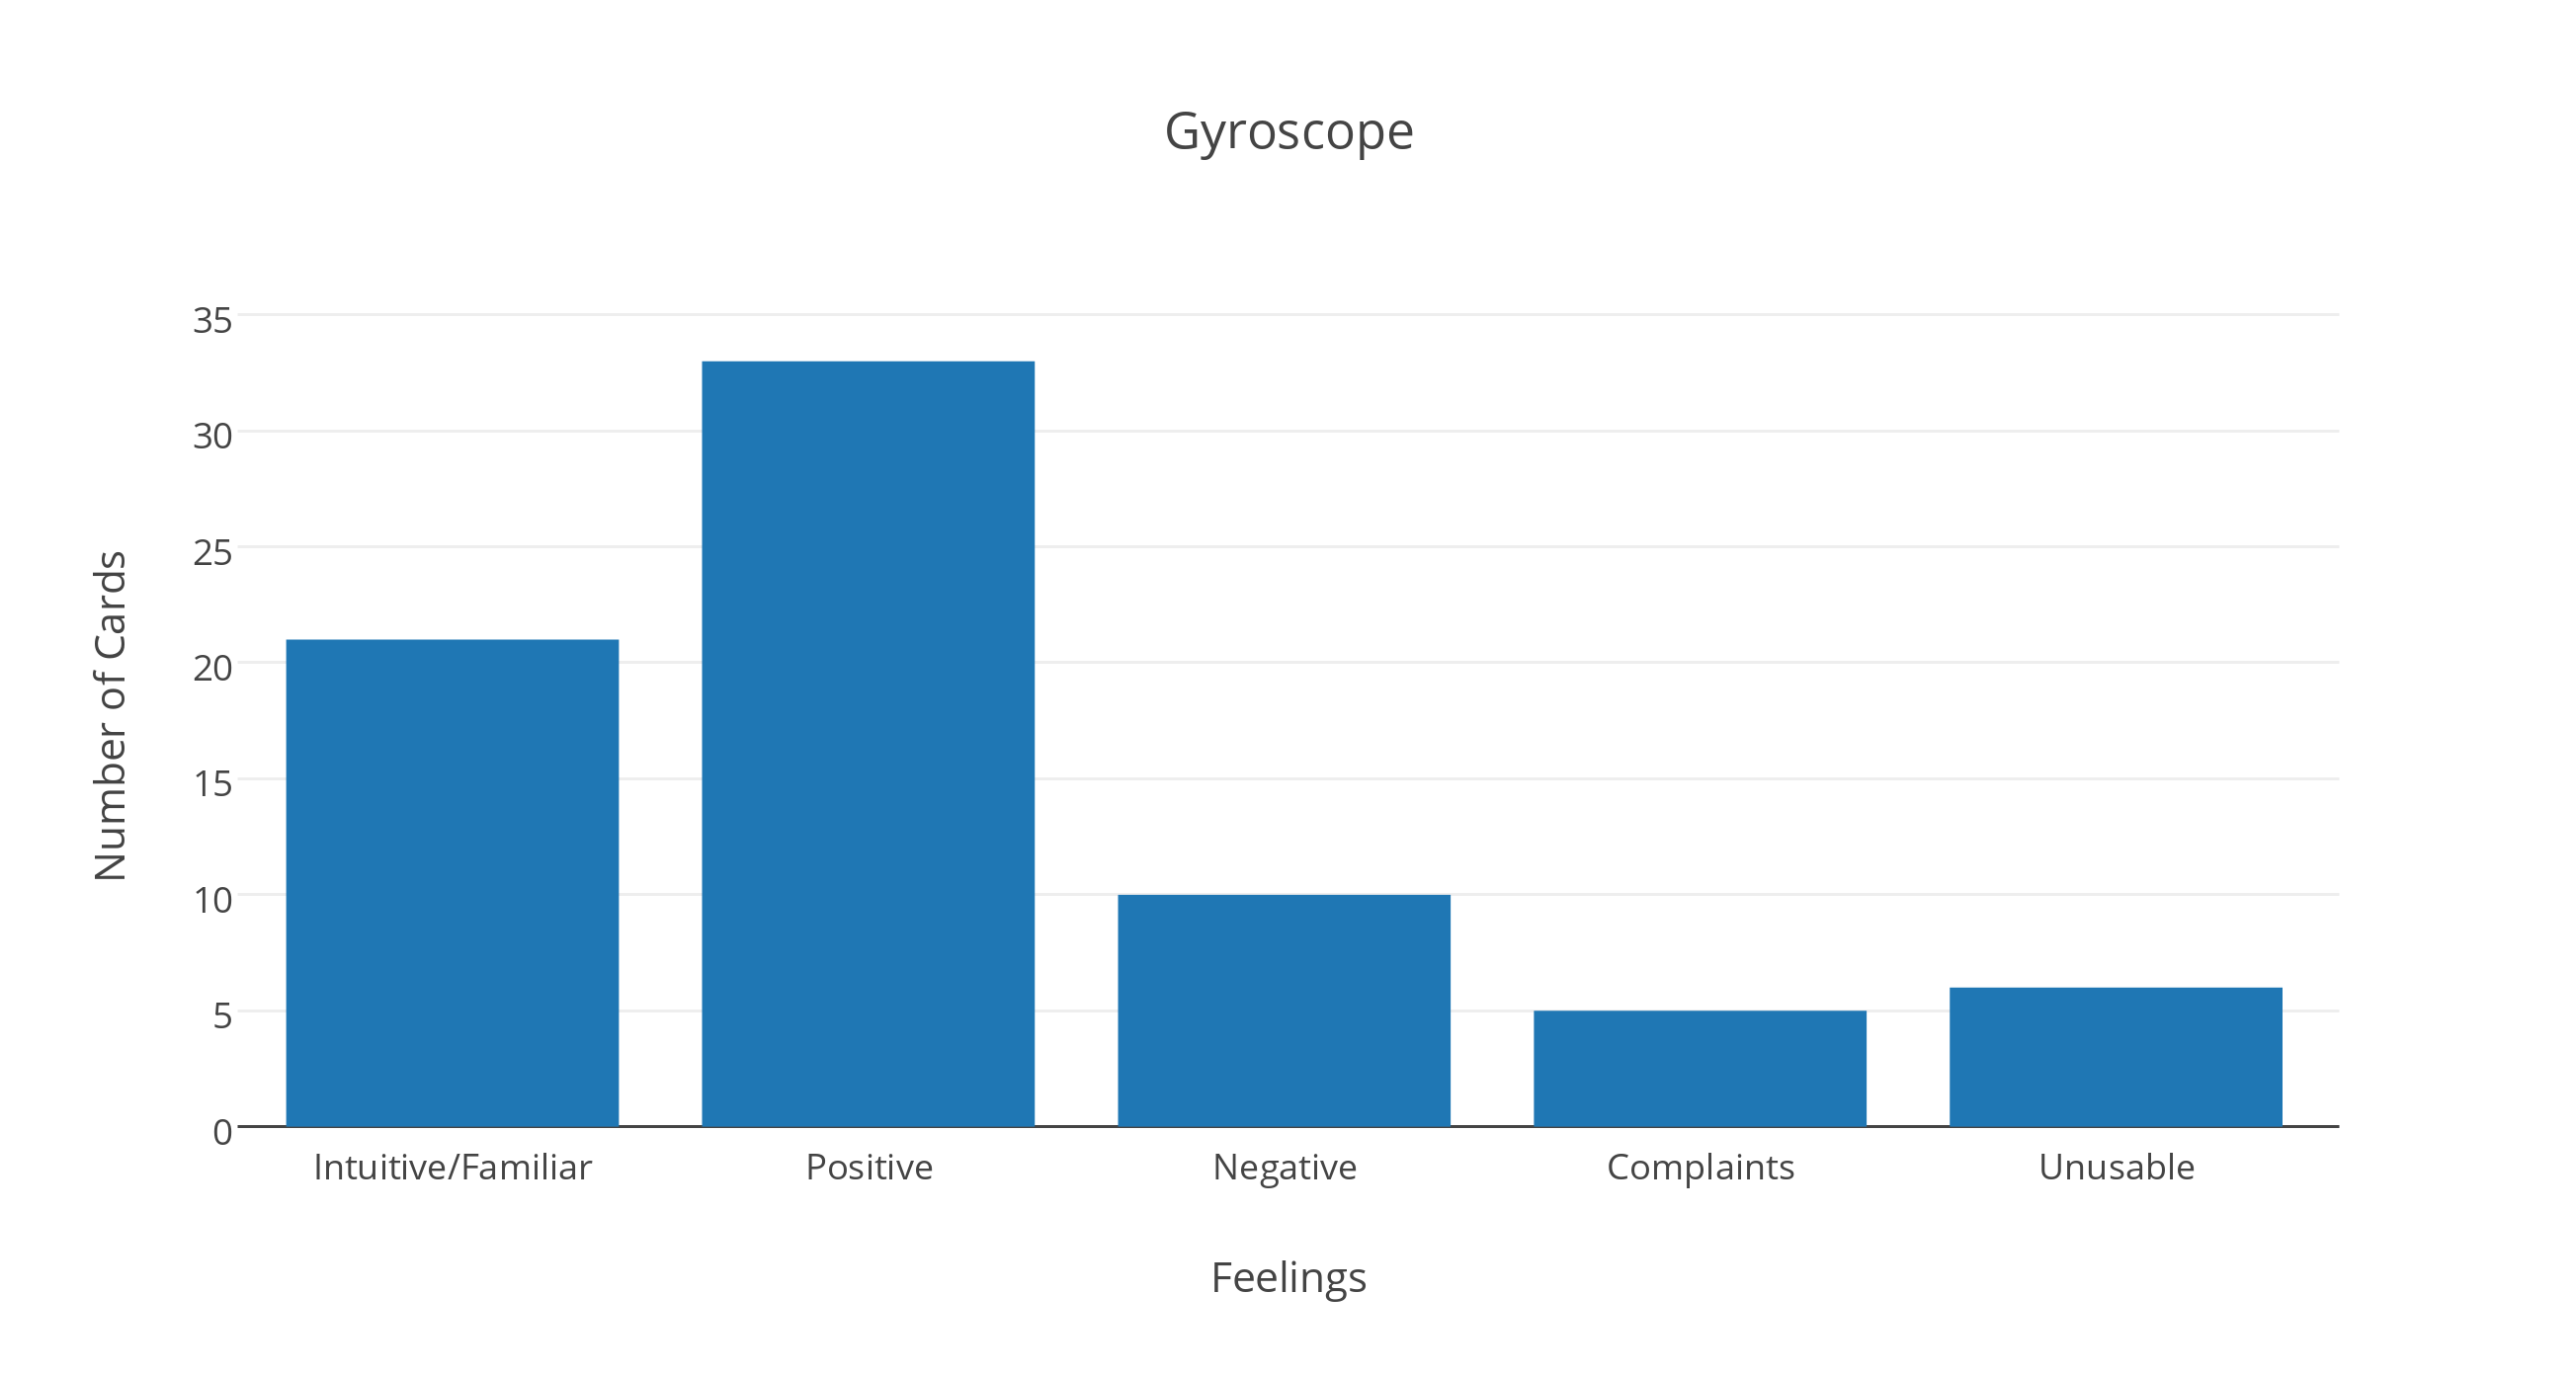
\includegraphics[scale=0.5]{Gyroscope.png}
\caption{Categorisation of the cards for the gyroscope control scheme.}
\end{figure}

\begin{figure}[H]
\centering
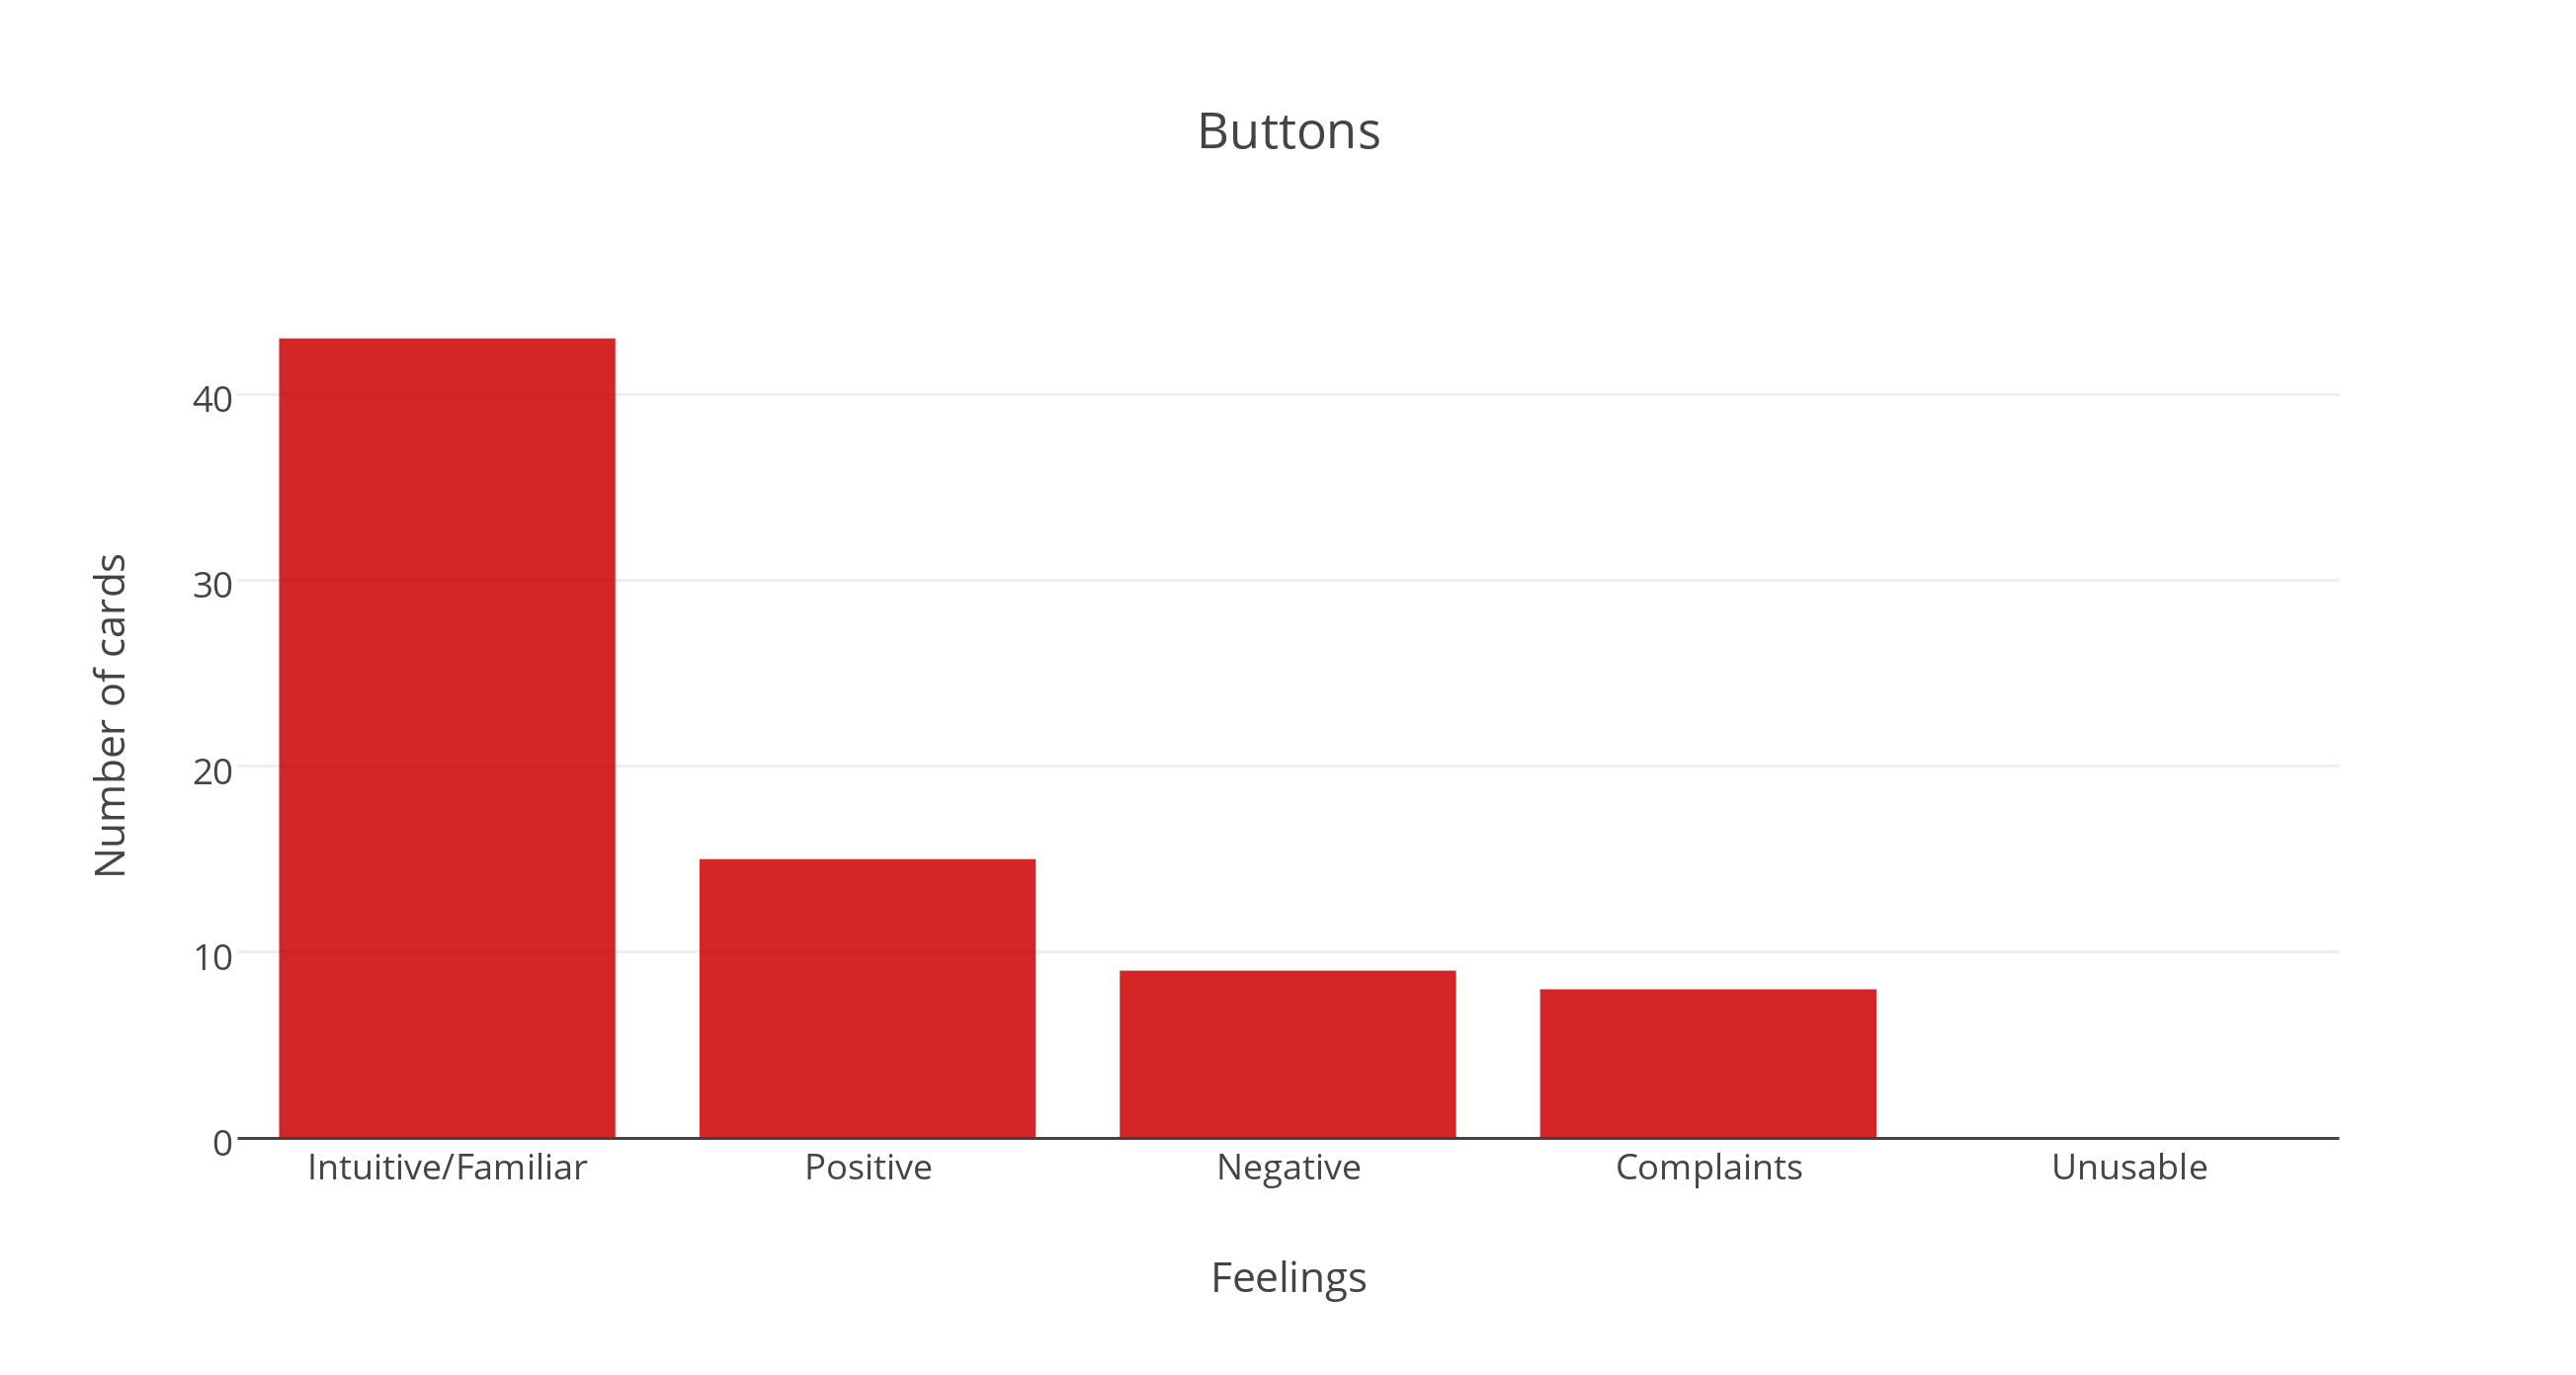
\includegraphics[scale=0.5]{Buttons.png}
\caption{Categorisation of the cards for the button control scheme.}
\end{figure}

\begin{figure}[H]
\centering
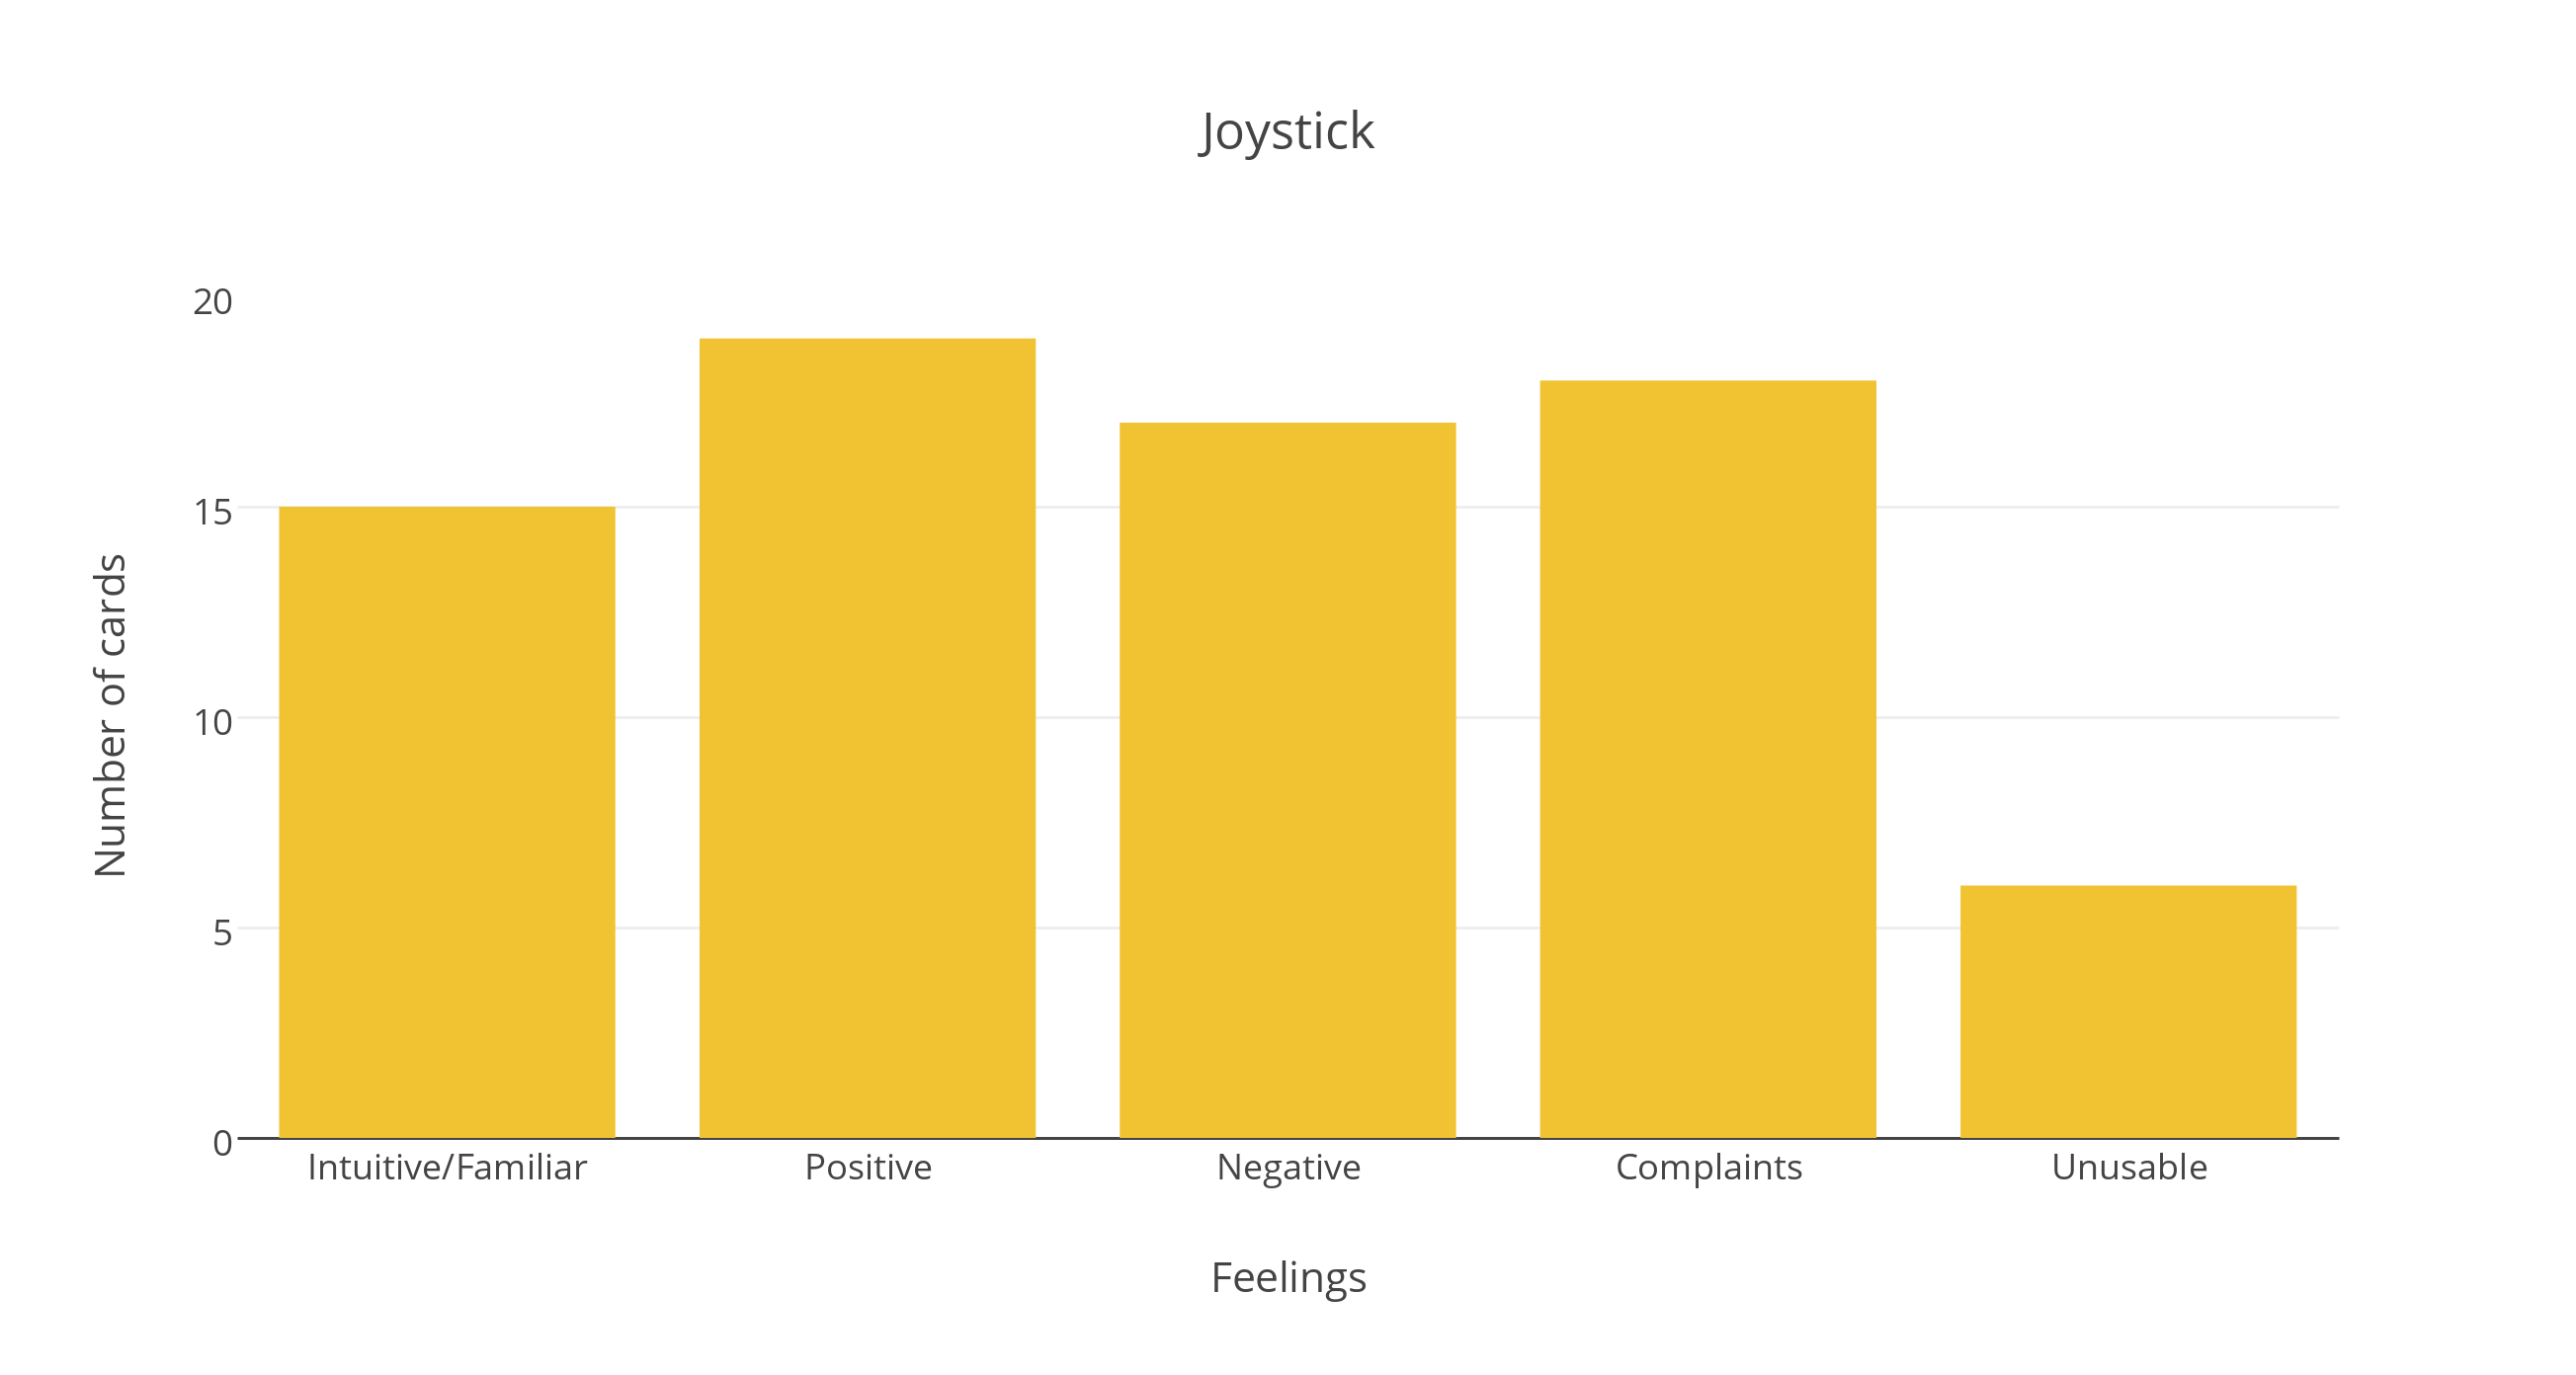
\includegraphics[scale=0.5]{Joystick.png}
\caption{Categorisation of the cards for the joystick control scheme.}
\end{figure}

write something about this ...

The time from the performance tests was calculated to find the mean and made graphs to visualize this as well. 

\begin{figure}[H]
\centering
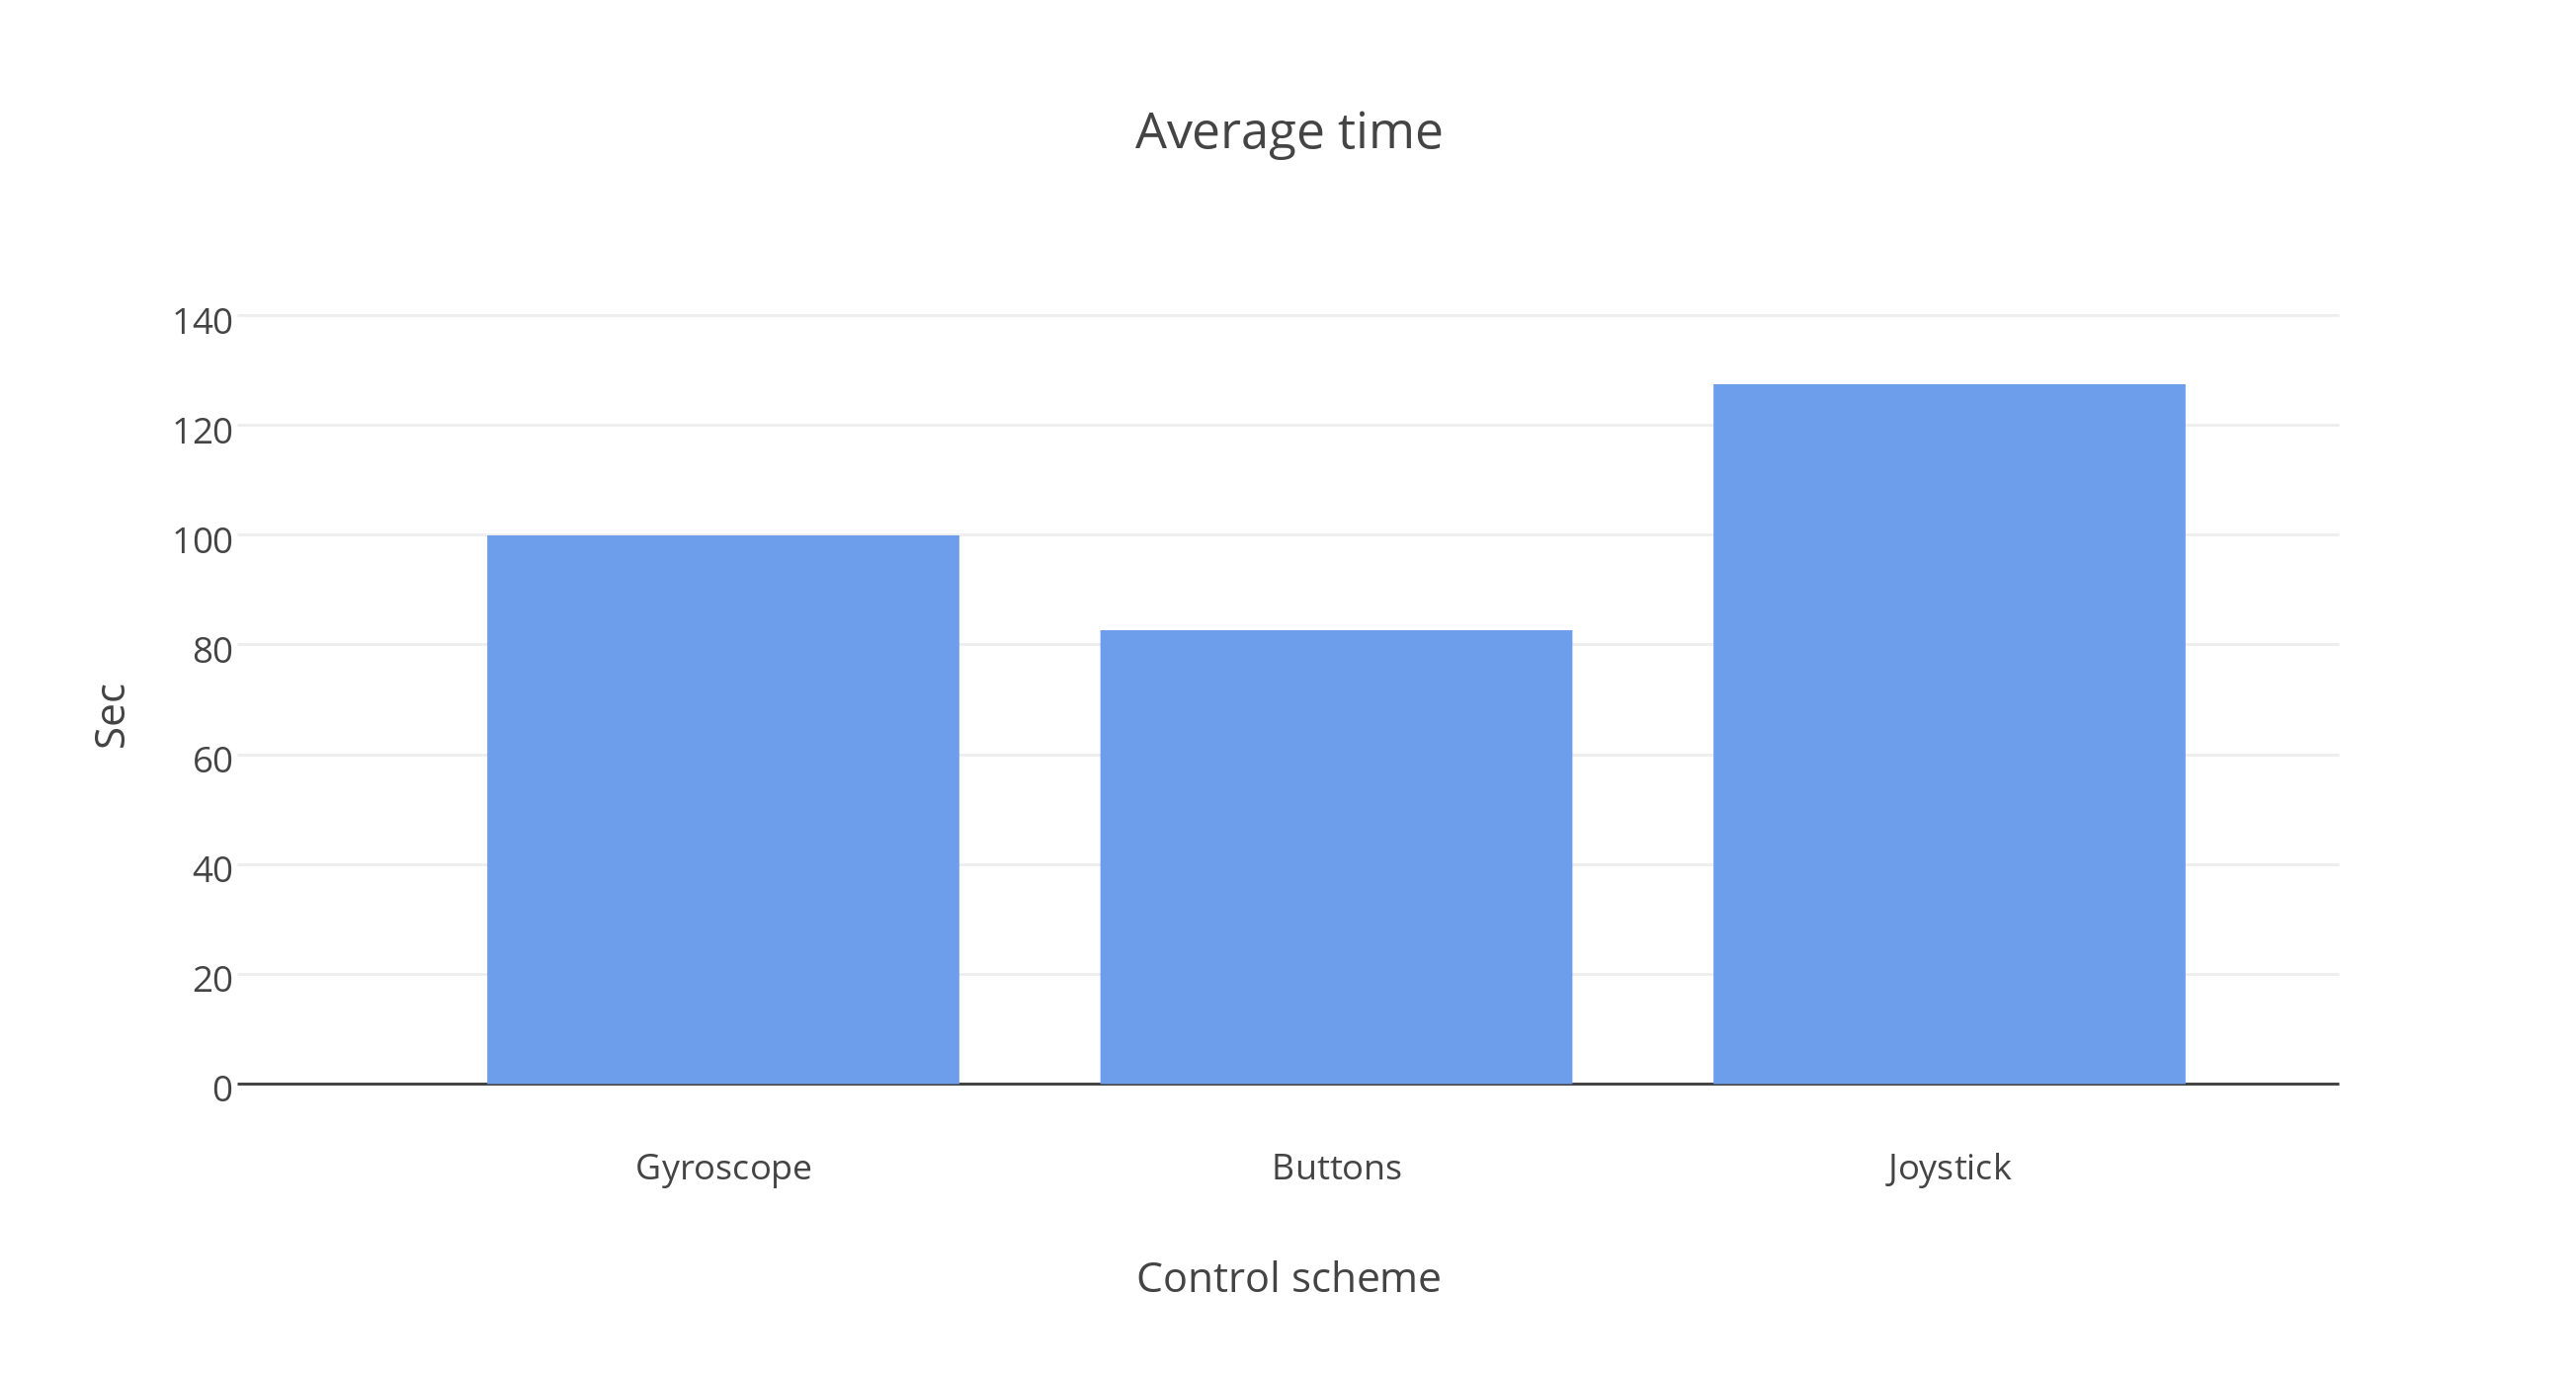
\includegraphics[scale=0.5]{Averagetime.png}
\caption{The average time it took for the participants to complete the level within the different comtrol schemes.}
\end{figure}

It is fairly easy to conclude that the buttons were the most efficient and the joystick the most problematic for our users. 


